\chapter{Baseline Pipeline}
\label{ch:baseline}

\noindent
This chapter outlines the baseline ETL pipeline that serves as a
control model for later evaluation. It demonstrates a minimal,
functional data workflow built with industry-standard components but
without any embedded governance or assurance features. The baseline
provides the empirical ground for measuring how DevSecOps practices
enhance auditability in the proposed system.

\section{Overview}
\noindent
The pipeline extracts public data from the SEC~EDGAR API, stages it to
Amazon~S3 as raw CSV, transforms it with Spark on~EMR, and writes
curated Parquet outputs to S3. Airflow, running on a Dockerised~EC2
instance, orchestrates the workflow. Infrastructure is deployed through
Terraform and continuously integrated with GitHub~Actions, which builds
the Airflow image, provisions resources, and triggers deployments on
each \texttt{push} to \texttt{main}.

\paragraph{Scope.}
The configuration is intentionally simple. It omits authentication
hardening, formal lineage capture, or immutability controls. Defaults
are accepted where possible to keep the environment lightweight,
reproducible, and comparable to the secured prototype that follows.

\section{Architecture}
\noindent
The system operates across three planes: orchestration, compute, and
storage. Figure~\ref{fig:baseline-architecture} shows the arrangement of
these components within AWS. Airflow on~EC2 acts as the control plane,
submitting Spark jobs to EMR and coordinating their execution. The data
plane spans two S3 buckets---one for raw ingestion and one for curated
outputs---linked by Spark transformations.

\begin{figure}[H]
  \centering
  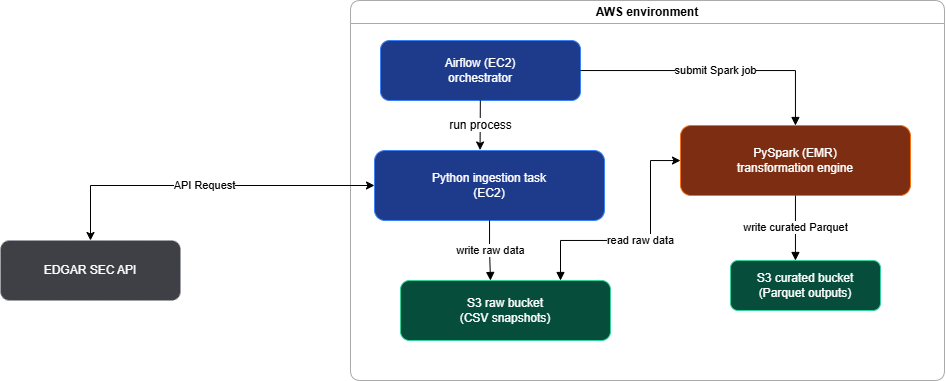
\includegraphics[width=0.9\textwidth]{diagrams/baseline_pipeline/arcitecture.png}
  \caption{Baseline runtime architecture showing orchestration,
  compute, and storage components.}
  \label{fig:baseline-architecture}
\end{figure}

\noindent
Continuous integration and deployment are automated through
GitHub~Actions. Figure~\ref{fig:baseline-cicd} illustrates the CI/CD
workflow: syntax checks precede infrastructure provisioning via
Terraform, after which the Airflow image---which embeds the DAGs---is
built, pushed to~GHCR, and redeployed to the EC2~host.

\begin{figure}[H]
  \centering
  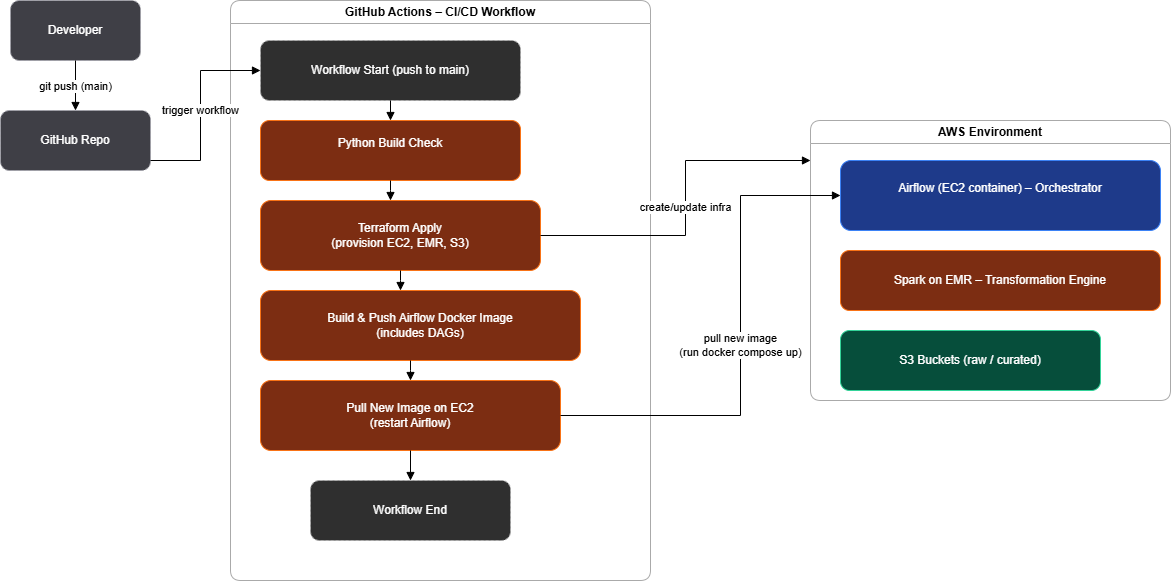
\includegraphics[width=0.9\textwidth]{diagrams/baseline_pipeline/ci_cd.png}
  \caption{CI/CD pipeline treated as a DAG within GitHub~Actions.}
  \label{fig:baseline-cicd}
\end{figure}

\section{Functionality}
\noindent
Figure~\ref{fig:baseline-dag} presents the Airflow~DAG that governs the
ETL workflow. A single linear sequence performs ingestion, submission
of Spark jobs, and post-run manifest recording.

\begin{figure}[H]
  \centering
  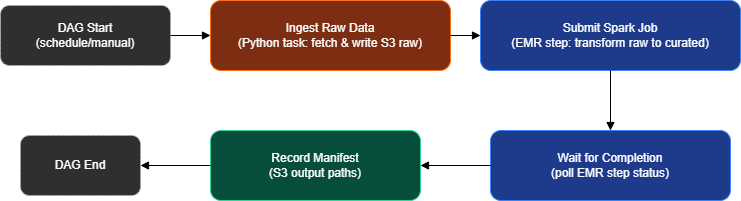
\includegraphics[width=0.85\textwidth]{diagrams/baseline_pipeline/airflow_dag.png}
  \caption{Baseline Airflow~DAG showing orchestration sequence.}
  \label{fig:baseline-dag}
\end{figure}

\noindent
Data moves through three primary stages (Figure~\ref{fig:baseline-data}).
The ingestion task fetches source files and stores them in the raw~S3
bucket. Spark reads these raw objects, enforces schema consistency,
cleans and deduplicates records, and writes Parquet datasets to the
curated bucket, partitioned by ingestion date. Each run emits a simple
manifest (\texttt{\_SUCCESS}) listing output paths for downstream
validation.

\begin{figure}[H]
  \centering
  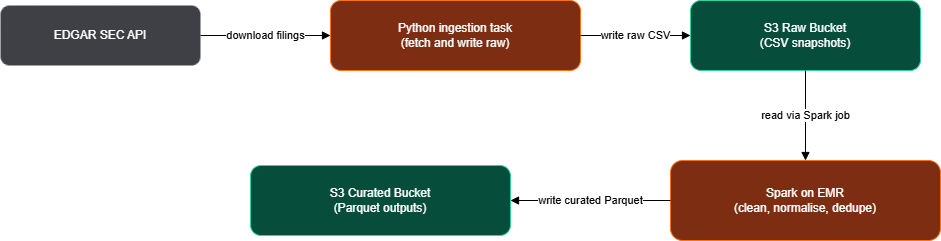
\includegraphics[width=0.85\textwidth]{diagrams/baseline_pipeline/data_path.png}
  \caption{Data path from ingestion to curated output in the baseline pipeline.}
  \label{fig:baseline-data}
\end{figure}

\section{Observed Gaps}
\noindent
While the baseline performs correctly, it lacks the controls required
for trustworthy audit evidence.

\paragraph{Lineage.}
Provenance is implicit in log files rather than captured as structured
metadata. No mapping links a specific input object, transformation
script, and output dataset.

\paragraph{Reproducibility.}
Environment state is defined by mutable container images. There is no
guarantee that a re-run reproduces prior results byte-for-byte, nor any
version pinning for dependencies or configuration.

\paragraph{Governance and Security.}
IAM policies are broad, and actions are not gated by review or policy
validation. Objects in S3 remain mutable and unsigned, and there is no
mechanism to detect tampering or verify artifact integrity.

\section{Summary}
\noindent
The baseline ETL pipeline demonstrates a functioning but ungoverned
data workflow. It provides consistent data movement from extraction to
curated storage, yet its assurance relies on convention rather than
design. The next chapter extends this model with explicit DevSecOps
controls---embedding lineage tracking, immutable evidence, and governed
infrastructure to meet auditability expectations.
